\documentclass[11pt]{article}
\usepackage[margin=1.05in]{geometry}
\usepackage{amsmath,amssymb,booktabs}
\usepackage{graphicx}
\usepackage[expansion=false]{microtype}
\usepackage[font=small,labelfont=bf,skip=5pt]{caption}
\usepackage[colorlinks=true,linkcolor=black,citecolor=black,urlcolor=blue]{hyperref}
\usepackage{titlesec}
\titlespacing{\section}{0pt}{1.4em}{0.5em}
\titlespacing{\subsection}{0pt}{1.0em}{0.35em}
\titlespacing{\subsubsection}{0pt}{0.8em}{0.3em}
\setlength{\parskip}{0.35em}
\renewcommand{\topfraction}{0.92}
\renewcommand{\bottomfraction}{0.75}
\renewcommand{\textfraction}{0.06}
\renewcommand{\floatpagefraction}{0.85}
\newcommand{\rs}{$r^{*}$}

\begin{document}

\begin{center}
{\large\textbf{Whose \boldmath$r^{*}$?}}\\[0.3em]
{\normalsize Belief Transmission, Intercept Disagreement, and the Price of Long Bonds}\\[0.6em]
{\small Dissertation prospectus \textperiodcentered\ 11 August 2026}
\end{center}
\vspace{0.2em}
\noindent\rule{\textwidth}{0.4pt}
\suppressfloats[t]

% =====================================================================
\section{The question}

The federal funds rate is an overnight rate. The ten-year Treasury yield is not, and its
thirty-year decline is usually attributed to forces outside monetary policy --- demographics,
productivity, the global supply of safe assets. Hillenbrand (2025) shows that this decline
accumulated almost entirely inside three-day windows around FOMC announcements, and argues
the Fed was revealing its own estimate of the long-run equilibrium rate.

That interpretation makes a specific structural claim that has not been examined. Write the
policy rule as
\begin{equation}
i_t \;=\; \underbrace{r^{*}_t + \pi^{*}_t}_{\text{intercept}} \;+\; \phi_\pi\!\left(\pi_t - \pi^{*}_t\right) + \phi_x x_t + v_t .
\label{eq:rule}
\end{equation}
\rs{} is the \emph{intercept} of the reaction function. So ``the Fed reveals \rs{}'' means the
Fed is telling markets about the constant in its own rule, and disagreement between the Fed
and the market about \rs{} is disagreement about that constant. This is a different object
from the one the literature has studied. Bauer, Pflueger \& Sunderam (2024) estimate the
market's perceived \emph{slope} $\phi_\pi$ from forecaster panels and show it prices term
premia; they absorb the intercept into forecaster fixed effects and say so explicitly. The
intercept has been assumed known, assumed common, or differenced away.

\begin{quote}
\textbf{This project asks: how does the Fed move beliefs about the intercept of its own
reaction function, and what does disagreement about that intercept do to the price of long
bonds?}
\end{quote}

\noindent The question decomposes into three parts, in increasing order of ambition:

\begin{enumerate}\setlength\itemsep{0.15em}
\item \textbf{Transmission.} Does the Fed's published longer-run projection move market
participants' beliefs about the long-run rate, and in which direction does causality run?
\item \textbf{Pricing.} Does the revision in beliefs about the intercept pass through to long
yields, and does it do so with the maturity signature of an endpoint shock rather than a
stance shock?
\item \textbf{Disagreement.} Is uncertainty about the intercept --- as opposed to its level ---
compensated in the term premium, and is the compensation asymmetric in the direction of the
perceived error?
\end{enumerate}

A second, methodologically independent component, described in \S7, asks a question the
first cannot answer and which requires none of its assumptions: \emph{why do only
scheduled-date price changes persist?}

% =====================================================================
\section{Three motivating facts}

All three are established on data already assembled: Gürkaynak--Sack--Wright zero-coupon
yields, the Adrian--Crump--Moench daily decomposition, a hand-built FOMC calendar of 300
scheduled meetings and 73 unscheduled actions covering June 1989 to July 2026, the SEP
dot-plot archive from January 2012, and the New York Fed Survey of Primary Dealers
longer-run federal funds rate from 2013.

\subsection{Fact 1: long yields fall only when the Fed is in the room}

Between June 1989 and June 2021 the ten-year yield fell 6.99 pp, of which 6.16 pp (88\%)
accrued inside three-day FOMC windows representing 11.8\% of trading days. Outside those
windows the drift is $-0.012$ bp/day with $t = -0.18$ across 7{,}035 days; a randomisation
test placing 324 randomly timed three-day blocks on non-FOMC days puts the observed figure at
the 0th percentile of 5{,}000 draws.

Extending to July 2026 --- a period no paper in this literature covers --- adds a fact that
constrains any mechanism. Over 2022--2026 the Fed raised the target 525 bp and the ten-year
rose 2.60 pp; inside FOMC windows it \emph{fell} 1.20 pp. The entire tightening in long rates
happened on non-FOMC days, and the in-window series continued to decline throughout
(Figure~\ref{fig:fact}).

\begin{figure}[tbp]
\centering
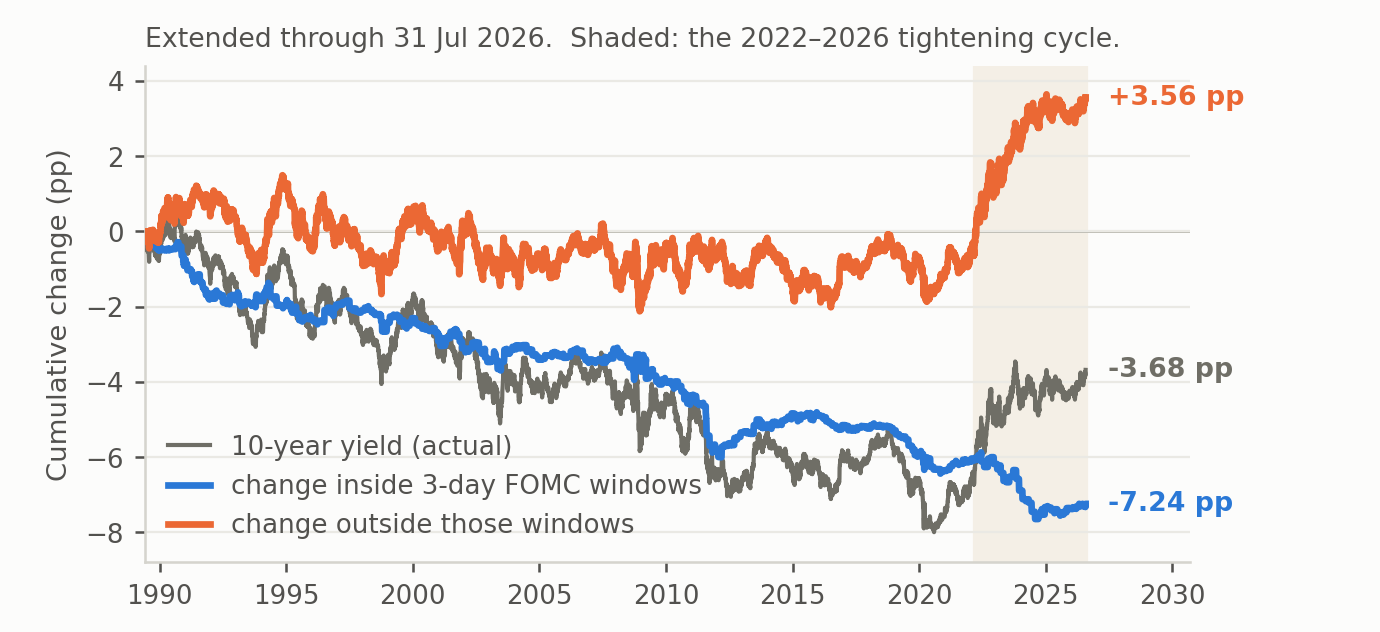
\includegraphics[width=0.95\textwidth]{s_extend.png}
\caption{\textbf{Fact 1.} Cumulative change in the ten-year yield from 2 June 1989, split into
the part accruing inside three-day FOMC windows and the part accruing on all other days,
through 31 July 2026. Shaded: the 2022--2026 tightening cycle.}
\label{fig:fact}
\end{figure}

\subsection{Fact 2: the two beliefs move together, and asymmetrically}

The FOMC publishes its longer-run federal funds projection four times a year; the New York Fed
surveys primary dealers for the same object roughly two weeks before every meeting. Netting
the 2\% inflation objective from both gives two directly comparable measures of \rs{} --- one
the Fed's, one the market's --- with no term-structure model anywhere in the construction.

Three things are true of them (Figure~\ref{fig:beliefs}). First, \textbf{they are never far
apart}: across 48 matched meetings the Fed-minus-dealer gap has a standard deviation of
0.105 pp and a range of $-0.11$ to $+0.30$ pp, exceeding 25 bp in absolute value at 4\% of
meetings. Second, \textbf{dealers move with the Fed nearly one-for-one}: regressing the dealer
revision on the Fed's revision at the preceding meeting gives $\beta = 0.82$ ($t = 6.86$).
Third, \textbf{the reverse relation is present but much weaker}: regressing the Fed's revision
on the dealer revision already known to it gives $\beta = 0.31$ ($t = 3.91$).

\begin{figure}[tbp]
\centering
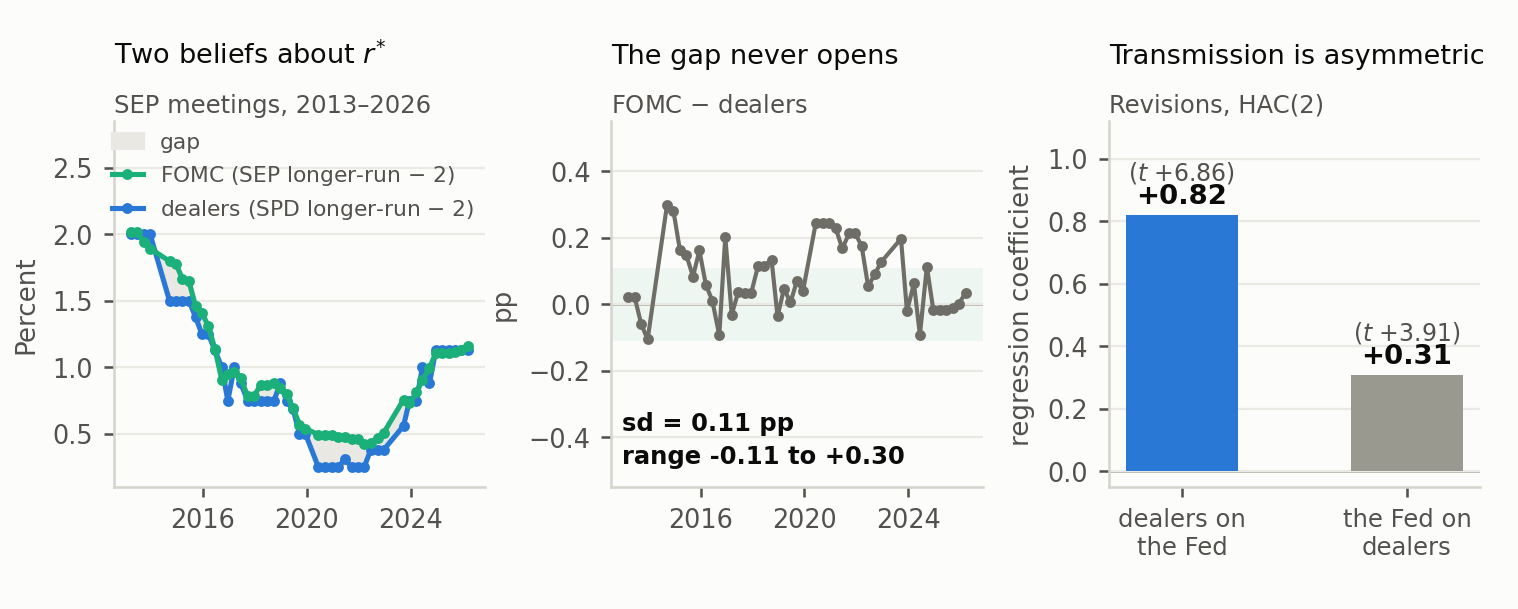
\includegraphics[width=0.98\textwidth]{s_beliefs.png}
\caption{\textbf{Fact 2.} Left: the FOMC's longer-run projection and the primary dealers'
longer-run federal funds rate, each less 2.0, at SEP meetings. Centre: the difference. Right:
revision regressions, HAC(2), 46--47 meetings.}
\label{fig:beliefs}
\end{figure}

The asymmetry is the interesting part, and it is not mechanical: both parties have the
opportunity to learn from the other, since the Desk briefs the FOMC with survey results before
each meeting. But the evidence stops short of a clean lead-lag. In a horse race the dealer
revision loads on both the preceding dot revision (0.60, $t=3.51$) and the contemporaneous one
(0.58, $t=3.23$), so part of what looks like following is anticipation --- unsurprising, since
the Fed's own revisions are serially correlated ($\rho = 0.38$, $t = 2.85$) while dealers' are
not ($\rho = -0.07$). \textbf{Establishing the direction of transmission at a frequency that
resolves this simultaneity is the first task of the project}, and it is what motivates the
high-frequency design in \S6.1.

\subsection{Fact 3: the phenomenon predates the measure}

Splitting the in-window drift by period gives $-2.46$ bp/meeting ($t=-3.06$) before 2012,
$-0.40$ ($t=-0.41$) from January 2012 to March 2022, and $-3.49$ ($t=-1.53$) thereafter. In
cumulative terms 81\% of the in-window decline is complete before the dot plot begins
(Figure~\ref{fig:timing}). In the decade when the FOMC cut its own longer-run rate by 1.78 pp
--- when an information channel should be loudest --- the in-window contribution is
indistinguishable from zero.

\begin{figure}[tbp]
\centering
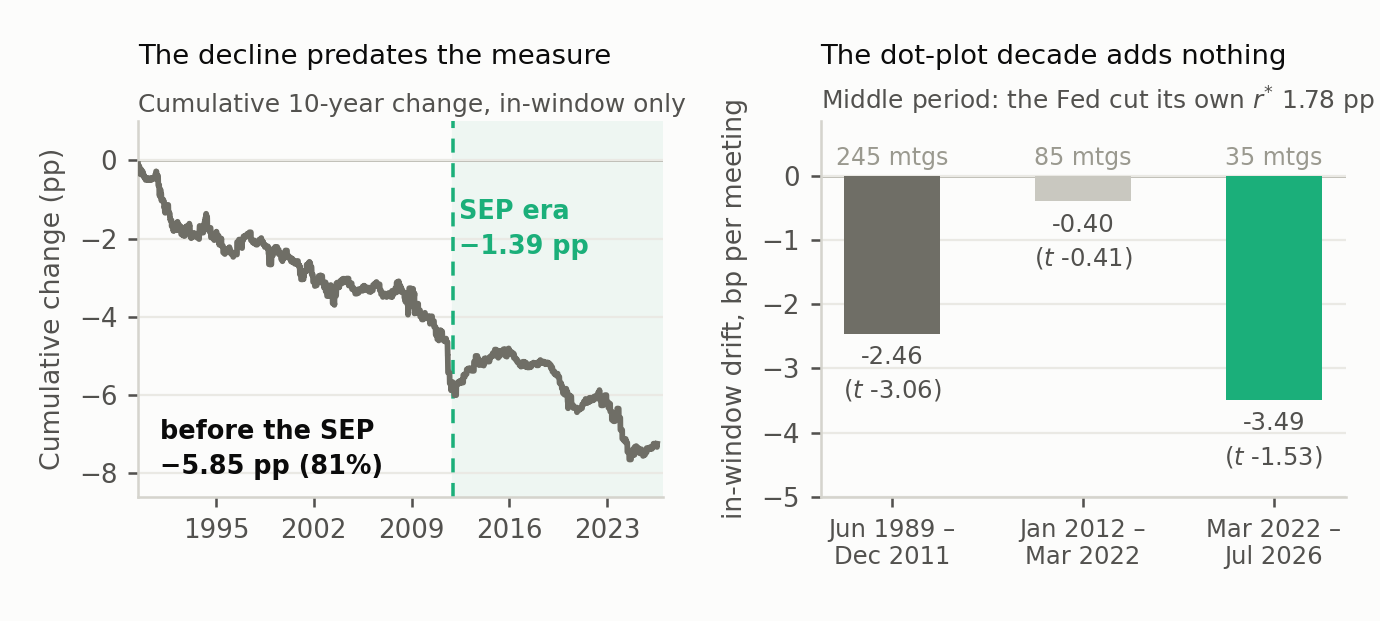
\includegraphics[width=0.95\textwidth]{s_timing.png}
\caption{\textbf{Fact 3.} Left: cumulative in-window decline in the ten-year yield with the SEP
era shaded. Right: in-window drift per meeting by period.}
\label{fig:timing}
\end{figure}

This is a binding constraint on the project rather than a puzzle to be explained away. It means
any design using the published projection is estimated on a sample where the yield response is
weak, and it is the reason the belief data --- rather than the yield data --- has to carry the
identification. It also motivates the contingent extension in \S9 using Tealbook projections,
which reach back to 1981.

% =====================================================================
\section{Framework}

\subsection{What a window response can contain}

Define the neutral nominal rate $i^{*}_t \equiv r^{*}_t + \pi^{*}_t$ and the policy gap
$\text{gap}_t \equiv i_t - i^{*}_t$, the stance of policy; under \eqref{eq:rule},
$\text{gap}_t = \phi_\pi(\pi_t-\pi^{*}_t) + \phi_x x_t + v_t$. Starting from the definition of
a long yield as an average of expected short rates plus a residual, and assuming the endpoints
are locally martingales,
\begin{equation}
y^{(n)}_t \;=\; r^{*}_t + \pi^{*}_t + \frac{1}{n}\sum_{j=0}^{n-1} E_t\!\left[\text{gap}_{t+j}\right] + TP^{(n)}_t .
\label{eq:identity}
\end{equation}
If the gap mean-reverts as an AR(1) with monthly persistence $\rho$, the expected-gap term is
$\omega(\rho,n)\,\text{gap}_t$ with $\omega(\rho,n) = (1-\rho^{n})/[n(1-\rho)]$, and the
analogous weight for a forward covering periods $n_1$ through $n_1+n_2-1$ is
$\omega^{f} = \rho^{n_1}(1-\rho^{n_2})/[n_2(1-\rho)]$. Differencing over an announcement
window,
\begin{equation}
\Delta y^{(n)}_t \;=\; \underbrace{\Delta r^{*}_t + \Delta \pi^{*}_t}_{\text{endpoint news}}
\;+\; \underbrace{\omega\,\Delta\text{gap}_t + \text{gap}_t\,\Delta\omega}_{\text{stance and persistence news}}
\;+\; \Delta TP^{(n)}_t .
\label{eq:windowdiff}
\end{equation}

Four terms, one observable. The claim that window moves are endpoint news requires all three
of the others to contribute approximately nothing, and each is a separate assumption. The
stance exclusion is usually defended by observing that the pattern survives in the 5-year,
5-year-forward rate, where $\omega^{f}$ is small. How small is an empirical question about
$\rho$:

\begin{center}\small
\begin{tabular}{lcccc}
\toprule
Half-life of the gap & $\omega$, 2-year & $\omega$, 5-year & $\omega$, 10-year & $\omega^{f}$, 5y5y\\ \midrule
1 year  & 0.56 & 0.29 & 0.15 & 0.01\\
2 years & 0.73 & 0.48 & 0.28 & 0.09\\
4 years & 0.85 & 0.67 & 0.48 & 0.28\\
\bottomrule\end{tabular}
\end{center}

\noindent Estimating an AR(1) on a crude gap proxy --- the one-year yield less HLW \rs{} plus 2
--- gives a half-life of 4.4 years on the full sample and 4.1 years post-1995. At that
persistence a 100 bp revision to the expected stance moves the ten-year about 50 bp and the
5y5y forward about 30 bp, so the far-forward evidence does not by itself separate endpoint
news from stance news. This is not a criticism the project needs to win in order to proceed;
it is the reason the project measures beliefs directly rather than inferring them from the
curve.

\subsection{The maturity signature}

Equation \eqref{eq:windowdiff} yields a test that requires no decomposition and no auxiliary
data. An endpoint shock enters $y^{(n)}$ with a coefficient of one at every maturity; a stance
shock enters with $\omega(\rho,n)$, which is strictly decreasing in $n$. So the \emph{shape} of
the window response across the maturity spectrum discriminates between them: flat in $n$ for
endpoint news, declining in $n$ for stance news, with a slope pinned down by $\rho$. Because
the discrimination comes from a cross-maturity restriction rather than a model of the pricing
kernel, it is immune to the critique in \S8.2.

\subsection{Two channels from intercept disagreement}

\textbf{Channel 1: uncertainty.} Dispersion in beliefs about the intercept propagates into the
variance of the entire expected policy path, undamped by horizon --- unlike stance
uncertainty, which is damped by $\omega$. Ahonon \& Roussellet (2025) estimate that investor
uncertainty about \rs{} is on the order of $\pm$170 bp, which makes the magnitude plausible.
The prediction is a term premium that rises with intercept dispersion and, critically, whose
sensitivity does \emph{not} decay with maturity.

\textbf{Channel 2: perceived policy error.} With $\delta \equiv r^{*m} - r^{*F}$, the market
evaluates the stance against its own neutral rate while the Fed sets policy against its own,
so the market perceives a stance $\delta$ away from the Fed's. Positive $\delta$ means policy
looks too easy: expected inflation overshoot, an expected later correction, and compensation
in the inflation dimension. Negative $\delta$ means policy looks too tight: expected
disinflation or recession, and compensation in the real dimension. The prediction is
\emph{asymmetric in the sign} and, more distinctively, asymmetric in \emph{which} risk is
compensated --- breakevens rising in one case and falling in the other. This is testable on
TIPS and nominal curves directly.

Fact 2 constrains this severely: the level of $\delta$ measured from published projections
never gets large. \S6.4 addresses what can be done about that, and \S9 states plainly what
would have to be true for the channel to remain testable.

\subsection{A minimal two-belief model}

The two channels can be stated in one pricing equation, and doing so delivers the
identification strategy rather than merely organising the intuition.

Let the Fed set policy against its own estimate $r^{*F}$ and let the representative investor
hold $r^{*m}$, with $\delta_t \equiv r^{*m}_t - r^{*F}_t$. The investor knows the rule, so his
expectation of the \emph{policy rate} uses the Fed's intercept; but he evaluates the
\emph{economy} using his own, so he perceives a stance $\delta_t$ looser than the Fed does.
If he believes policy that is $\delta$ too easy raises inflation, and that the Fed will
eventually respond, his expected path carries a correction term:
\begin{equation}
E^{m}_t\!\left[i_{t+j}\right] \;=\; r^{*F}_t + \pi^{*}_t + \rho^{\,j}\,\text{gap}_t \;+\; \lambda_j\,\delta_t ,
\label{eq:twobelief}
\end{equation}
where $\lambda_j$ is the perceived-correction profile: near zero at short horizons, since the
Fed is not about to change course; positive and peaking at business-cycle horizons as the
perceived error accumulates and is corrected; and returning to zero at long horizons, since the
correction is temporary. Averaging \eqref{eq:twobelief} and adding a premium gives
\begin{equation}
y^{(n)}_t \;=\; \underbrace{r^{*F}_t + \pi^{*}_t}_{\text{endpoint}} \;+\; \underbrace{\omega(\rho,n)\,\text{gap}_t}_{\text{stance}} \;+\; \underbrace{\Lambda(n)\,\delta_t}_{\text{perceived error}} \;+\; \underbrace{TP^{(n)}\!\left(\sigma^2_{\delta,t}\right)}_{\text{disagreement premium}} ,
\label{eq:pricing}
\end{equation}
with $\Lambda(n) = n^{-1}\sum_{j<n}\lambda_j$.

The empirical content is that the four terms have \emph{four different maturity profiles}:

\begin{center}\small
\begin{tabular}{@{}llp{0.40\textwidth}@{}}
\toprule
\textbf{Term} & \textbf{Loading on $n$} & \textbf{Shape}\\ \midrule
Endpoint news $\Delta r^{*F}$ & $1$ & flat at every maturity\\
Stance news $\Delta\text{gap}$ & $\omega(\rho,n)$ & strictly decreasing, slope set by $\rho$\\
Perceived error $\delta$ & $\Lambda(n)$ & hump-shaped: small at 1--2 years, peaking at intermediate maturities, decaying at the long end\\
Disagreement premium & increasing in $n$ & rising, and \emph{not} decaying --- the signature that separates it from every damped uncertainty measure\\
\bottomrule\end{tabular}
\end{center}

\noindent Two further restrictions come free. First, the perceived-error term is the only one
that predicts \emph{curvature} in the response --- so a hump in the estimated maturity profile
is direct evidence of a perceived policy error, and its absence is evidence against. Second,
$\delta$ enters expected inflation and the expected real path with opposite signs: if policy
is perceived too easy, breakeven inflation should rise while the real forward falls at the
correction horizon, and the reverse if policy is perceived too tight. So the \emph{split} of
the response between the nominal and TIPS curves identifies the sign channel without any
decomposition of the nominal curve itself. This is the empirical content of \S6.2 and \S6.4.

% =====================================================================
\section{Relation to the literature}

\begin{center}\footnotesize
\begin{tabular}{@{}p{0.30\textwidth}p{0.30\textwidth}p{0.34\textwidth}@{}}
\toprule
\textbf{Paper} & \textbf{Object} & \textbf{What it leaves open}\\ \midrule
Hillenbrand (2025, \emph{RFS}) & Window decline is endpoint learning & Never tests the exclusions; no belief data\\[0.3em]
Bauer, Pflueger \& Sunderam (2024, \emph{QJE}) & Perceived \emph{slope} $\phi_\pi$ from forecaster panels; prices term premia & Absorbs the intercept into forecaster fixed effects, explicitly\\[0.3em]
Bauer \& Rudebusch (2020, \emph{AER}) & \rs{} \emph{level} in an arbitrage-free model & A single trend, not two contested beliefs\\[0.3em]
Cao, Crump, Eusepi \& Moench (SR 934) & Forecaster-vs-forecaster disagreement about the long-run level; $\sim$1/3 of TP variation & Unsigned; not Fed-vs-market; requires an affine model\\[0.3em]
Caballero \& Simsek (2022, \emph{AER}) & Fed-market disagreement $\to$ sign-dependent policy risk premium & Disagreement is about \emph{demand}, which mean-reverts; no term structure, no TIPS\\[0.3em]
Cieslak \& McMahon; Cieslak, McMahon \& Pang & Perceived policy errors raise term premia; WSJ-text measure & Error is about the state and the slope, never the intercept\\[0.3em]
Bauer, Lakdawala \& Mueller (2022, \emph{EJ}) & Option-implied policy uncertainty, 1--2 year horizon & Silent on \rs{}; a control, not a competitor\\[0.3em]
Ahonon \& Roussellet (SR 1187) & Investor uncertainty about \rs{} priced in bonds & Representative investor; no Fed-vs-market object\\
\bottomrule\end{tabular}
\end{center}

\vspace{0.4em}
\noindent Three elements appear to be unclaimed: disagreement that is \emph{Fed-versus-market}
rather than forecaster-versus-forecaster; a \emph{signed} gap rather than a dispersion measure;
and the mapping from the sign to \emph{which} risk is compensated. The SEP \emph{longer-run}
dot as an asset-price regressor is also effectively unused --- work using the SEP uses
near-term dots or lift-off timing.

Two positioning risks require explicit treatment in any draft. Caballero \& Simsek already have
a sign-dependent policy risk premium from Fed-market disagreement; the defence is that
intercept disagreement is permanent and horizon-invariant whereas demand disagreement
mean-reverts, which is exactly what generates the distinctive non-decaying maturity signature
in \S3.2. And Cao et al.\ already price long-run-level disagreement, which is why the project
should lead with transmission and the maturity signature rather than with a dispersion result.

% =====================================================================
\section{Data}

\begin{itemize}\setlength\itemsep{0.1em}
\item \textbf{Yields.} GSW zero-coupon nominal curve, 1--30 years, daily 1961--2026; GSW TIPS
curve from 1999 (usable from roughly 2003); implied breakevens.
\item \textbf{Decompositions.} ACM daily risk-neutral and term-premium series, used only for
comparison with the literature, for the reasons in \S8.2.
\item \textbf{Events.} 300 scheduled FOMC meetings and 73 conference calls and unscheduled
actions, June 1989 -- July 2026, assembled from Federal Reserve historical meeting pages, with
SEP-release meetings flagged.
\item \textbf{The Fed's belief.} SEP longer-run federal funds projections, 57 meetings from
January 2012, at participant level: mean, median, cross-participant standard deviation and
interquartile range.
\item \textbf{The market's belief.} NY Fed Survey of Primary Dealers longer-run federal funds
rate, 92 surveys from 2013, with 25th and 75th percentiles; Survey of Market Participants from
2014; merged into the Survey of Market Expectations from 2025.
\item \textbf{To be added.} Intraday Treasury futures for the high-frequency design; Treasury
auction calendar for the issuance control; Blue Chip Financial Forecasts long-range;
Tealbook/Greenbook longer-run projections (five-year lag, available to 2019).
\end{itemize}

% =====================================================================
\section{Component A: transmission, pricing, and disagreement}

\subsection{A1. Does the longer-run projection move beliefs, and who leads?}

The survey evidence in Fact 2 cannot separate following from anticipation, because both series
are observed eight times a year and the Fed's revisions are persistent. Two designs sharpen it.

\emph{The SEP/non-SEP contrast.} The longer-run dot is published at four meetings a year and
not at the other four. If long-run guidance operates through the projection, the in-window
response of long yields should be larger at SEP meetings, and larger still at SEP meetings
where the longer-run dot moved. This is a within-Fed comparison that holds the announcement
format fixed, and it is estimable immediately on assembled data:
\begin{equation}
\Delta y^{(n)}_t \;=\; \alpha + \beta_1 \text{SEP}_t + \beta_2 \left(\text{SEP}_t \times |\Delta \text{dot}^{LR}_t|\right) + \gamma' Z_t + \varepsilon_t ,
\label{eq:sep}
\end{equation}
with $Z_t$ containing the Kuttner (2001) target surprise, the path factor, and pre-meeting
controls in the spirit of Bauer \& Swanson (2023).

\emph{The high-frequency window.} On SEP meetings the projections are released with the
statement, and the press conference follows. Intraday Treasury futures around each release let
the response to the longer-run projection be separated from the response to the near-term path
and from the press conference, which no work using the longer-run dot has done.

\emph{Falsification.} If $\beta_2$ is zero, the published endpoint does not move prices and
the transmission story is limited to the pre-2012 implicit channel --- which is testable only
with Tealbook data, and becomes the project's main contingency.

\subsection{A2. Does the belief revision have the maturity signature of an endpoint shock?}

Estimate the window response at every GSW maturity from 1 to 30 years, on the subsample of
meetings where the longer-run projection was revised, and test the cross-maturity restriction
in \S3.2: flat loading for endpoint news against $\omega(\rho,n)$ for stance news, with $\rho$
estimated from the gap process and also treated as a free parameter. This is a shape test on
a single curve, so it survives every criticism of the decomposition literature. The same test
run on the TIPS curve isolates the real endpoint and removes the $\Delta\pi^{*}$ term of
\eqref{eq:windowdiff} entirely.

\subsection{A3. Is disagreement about the intercept priced?}

Unlike the level gap, dispersion varies usefully: the dealer interquartile range of the
longer-run rate spans 0 to 0.75 pp, and the FOMC's own cross-participant standard deviation
spans 0.22 to 0.46 pp. Two specifications:

\begin{itemize}\setlength\itemsep{0.1em}
\item \emph{Level.} Regress long-horizon forward term premia on intercept dispersion,
orthogonalised against the Bauer--Lakdawala--Mueller option-implied policy uncertainty measure
(which is a 1-to-2-year object and publicly available) and against the forecaster dispersion
used by Cao et al.
\item \emph{State dependence.} Interact pre-meeting dispersion with the announcement surprise,
in the Bauer--Pflueger--Sunderam design but with the intercept in place of the slope.
\end{itemize}

The distinctive prediction, and the one that separates intercept dispersion from every existing
uncertainty measure, is that the sensitivity should \emph{not} decay with maturity.

\subsection{A4. Is the response asymmetric in the sign of the perceived error?}

This is the highest-risk element and Fact 2 has already ruled out its simplest version: with a
Fed-minus-dealer gap whose standard deviation is 10 bp, a signed level regressor has no usable
variation. Three routes remain, in descending order of my confidence:

\begin{enumerate}\setlength\itemsep{0.15em}
\item \textbf{Revision direction rather than level.} Test whether upward and downward revisions
to the longer-run projection have different pass-through to breakevens versus TIPS. This uses
the flow rather than the stock and has more variation, though power is limited --- 18 upward
revisions gives 21--31\% power against plausible effect sizes.
\item \textbf{Distributional gaps.} The Fed publishes the full distribution of participants'
longer-run dots and the SPD publishes response percentiles. Tail disagreement may be
substantially larger than median disagreement even when the medians coincide.
\item \textbf{The pre-2012 sample.} Tealbook longer-run projections against contemporaneous
Blue Chip long-range forecasts, where the disinflation and the productivity boom plausibly
generated genuine level disagreement, and where the yield response actually lives.
\end{enumerate}

% =====================================================================
\section{Component B: why only scheduled-date changes persist}

Component A rests on a chain of maintained assumptions. Component B rests on almost none, and
is the part of the project I would defend first.

Window and non-window days have nearly identical daily volatility --- 6.72 versus 5.60 bp ---
but completely different cumulative outcomes: $-6.16$ pp against $-0.82$ pp over the paper
sample. The drift-to-noise ratio is roughly 45 times higher inside the window. Announcement
days are not noisier days; they are days on which the noise does not cancel. So the question
is not which component of the yield moves, but why only scheduled-date price changes persist.

\emph{Design.} A long-horizon variance-ratio decomposition estimated separately by day type
converts this from a description into a measured object: the permanent share of a day's
innovation, estimated for window and non-window days at horizons from one month to two years,
with block-bootstrapped standard errors. It requires no decomposition, no endpoint measure and
no model of the term premium, so it survives every identification problem in Component A. It
also confronts Hanson, Lucca \& Wright (2021) --- who find announcement-window moves largely
reverse --- with Hillenbrand, who requires that they do not, on a statistic neither reports.

\emph{The competing explanation, and a decisive test.} Lou, Pintér, Üslü \& Walker (BIS WP
1232) document supply-driven pre-announcement drift in UK gilts and claim the effect
concentrates in FOMC windows \emph{without} long-dated Treasury issuance. If correct, the
mechanism is dealer inventory rather than monetary policy, and much of the literature is
misattributed. Auction dates are public. This test is a few days' work and it is decisive
either way, which is why it is scheduled first.

% =====================================================================
\section{Completed work}

Four results are finished and require no further data.

\subsection{The literature's disagreement about the channel is an event-list artifact}

Two circulating papers give opposite answers to whether the window decline is expectations or
term premium. I reproduce Pan \& Peng's day-$(t-1)$ estimates on their specification to three
coefficients ($-0.785$ / $-0.716$ / $-0.070$ against their $-0.79$ / $-0.71$ / $-0.08$) and
then show the attribution is not robust: the term-premium share moves from 91\% to 46\% on the
same day, same data and same decomposition, purely by changing the event list. The 73
conference calls and unscheduled actions a scheduled-only filter removes carry $-1.78$ pp of
expectations decline on day $t-1$ alone --- $-2.5$ bp per event against $-0.07$ bp for
scheduled meetings. Neither paper discusses the event list.

\subsection{The standard decomposition cannot arbitrate}

In a spanned affine model the expectations component is a fixed linear function of the curve,
$\Delta rn^{(n)}_t = c_n' \Delta y^{\mathcal N}_t$ with $c_n' = b_n' \mathbf{B}^{-1}$;
empirically $R^2 = 1.00000$ over 9{,}282 daily observations. Event responses therefore satisfy
$\beta^{rn} = c'\beta^{\mathcal N}$ exactly --- predicted $+2.5$ and $+29.3$ bp against directly
estimated $+2.6$ and $+29.2$ --- so the decomposition adds no event-specific information. And
$c'\mathbf{1} = 0.529$: a permanent, fully credible parallel shift is reported as 53\%
expectations and 47\% term premium. The algebra is a corollary of Joslin, Singleton \& Zhu
(2011) and the bias is Bauer \& Rudebusch (2020); the contribution is the explicit filter for
ACM and the event-study corollary.

\subsection{The effect and the measurement do not overlap in time}

Fact 3 above: 81\% of the in-window decline predates the dot plot.

\subsection{Neither candidate market-side \rs{} measure is usable}

The ACM 9-year, 1-year-forward risk-neutral rate loads 0.287 on the one-year yield with
$R^2 = 0.83$ and a level correlation of $+0.984$; it is a damped copy of the policy cycle, and
under a stationary VAR no forward horizon isolates an endpoint. The survey measure fails for
the opposite reason: dealers load 0.82 on the Fed's own revision, so it is contaminated by the
signal it is meant to price. One is circular with yields, the other with the Fed. This closes
the Fed-market wedge design rather than leaving it open, and it is a reportable negative
result.

% =====================================================================
\section{Risks and what would kill each component}

\begin{itemize}\setlength\itemsep{0.15em}
\item \textbf{Power in the SEP era.} 57 meetings, of which four a year publish the longer-run
dot, in a decade where the in-window yield response is $-0.40$ bp/meeting with $t=-0.41$. If
A1 returns a null, the honest conclusion is that the published endpoint does not move prices,
and the project pivots to Component B plus the Tealbook extension.
\item \textbf{Simultaneity.} Fact 2 shows transmission runs both ways. Without intraday data
the direction is not identified, so intraday futures are a prerequisite rather than a
refinement.
\item \textbf{The signed channel may be untestable.} If distributional gaps are as small as
median gaps and Tealbook access does not materialise, A4 should be dropped rather than
estimated on 18 events.
\item \textbf{Positioning.} If Caballero \& Simsek's empirical work already uses the longer-run
dot --- which I have not been able to verify --- the contribution narrows to the maturity
signature and the TIPS asymmetry. This needs checking before drafting.
\end{itemize}

% =====================================================================
\section{Timeline}

\begin{center}\small
\begin{tabular}{@{}llp{0.52\textwidth}@{}}
\toprule
\textbf{Period} & \textbf{Component} & \textbf{Task}\\ \midrule
Weeks 1--4 & B & Issuance test against the Treasury auction calendar; decisive either way\\
Weeks 1--6 & --- & Draft the event-list reconciliation note (\S8.1 plus \S8.3): self-contained, model-free, publishable now\\
Weeks 4--10 & A1 & SEP/non-SEP contrast on assembled data; acquire intraday futures\\
Weeks 8--16 & A2 & Maturity-signature test on nominal and TIPS curves\\
Term 2 & B & Variance-ratio decomposition by day type --- the intended chapter\\
Term 2 & A3 & Dispersion and term premia, orthogonalised against existing uncertainty measures\\
Contingent & A4 & Tealbook extension to the pre-2012 sample, subject to archive access\\
\bottomrule\end{tabular}
\end{center}

% =====================================================================
\section{Requests}

\begin{enumerate}\setlength\itemsep{0.1em}
\item Guidance on whether the reconciliation in \S8.1 is better as a standalone short
submission or as a methodological section of the main chapter.
\item Access to Blue Chip Financial Forecasts long-range and to the Tealbook archive. Both
bind on A4, which is the only route to testing any projection-based mechanism on the sample
that contains the phenomenon.
\item A view on the balance between Components A and B. Component B is the safer chapter and
the one I would defend; Component A is the one with a genuinely open position in the
literature. I do not think both can be first.
\end{enumerate}

\vspace{0.8em}
\noindent\rule{\textwidth}{0.4pt}\\[0.3em]
\footnotesize\textbf{References cited.} Ahonon \& Roussellet, FRBNY SR 1187. Adrian, Crump \&
Moench (2013), \emph{JFE}. Bauer, Lakdawala \& Mueller (2022), \emph{EJ} 132(644). Bauer,
Pflueger \& Sunderam (2024), \emph{QJE} 139(4). Bauer \& Rudebusch (2020), \emph{AER} 110(5);
(2014), \emph{IJCB}. Bauer \& Swanson (2023), \emph{NBER Macro Annual}. Caballero \& Simsek
(2022), \emph{AER} 112(7); NBER WP 30132. Cao, Crump, Eusepi \& Moench, FRBNY SR 934. Cieslak
\& McMahon, SSRN 4560220. Cieslak, McMahon \& Pang, SSRN 4920858. Gürkaynak, Sack \& Wright
(2007). Hanson, Lucca \& Wright (2021), \emph{QJE} 136(3). Hillenbrand (2025), \emph{RFS}
38(4). Hofmann, Li \& Wu, BIS WP 1252. Joslin, Priebsch \& Singleton (2014), \emph{JF}. Joslin,
Singleton \& Zhu (2011), \emph{RFS}. Kuttner (2001), \emph{JME}. Lou, Pintér, Üslü \& Walker,
BIS WP 1232. Pan \& Peng, SSRN 4764451. Rungcharoenkitkul \& Winkler (2025), \emph{JME}.

\end{document}
